\section{Tuần 7: Biến đổi Fourier và Lọc ảnh trong Miền Tần số}
\label{sec:week7}

Các câu hỏi trong tuần này dựa trên Bài giảng số 7 (\emph{Fourier Transform})~\citep{xlav_lec7}. Ký hiệu theo bài giảng: ảnh $f(x, y)$ kích thước $M \times N$; biến đổi Fourier rời rạc (DFT) và biến đổi ngược (trang 16)
\begin{equation}
F(u, v) = \frac{1}{MN}\sum_{x=0}^{M-1}\sum_{y=0}^{N-1} f(x, y)\,e^{-2\pi i\left(\frac{xu}{M} + \frac{yv}{N}\right)}, \qquad
f(x, y) = \sum_{u=0}^{M-1}\sum_{v=0}^{N-1} F(u, v)\,e^{2\pi i\left(\frac{xu}{M} + \frac{yv}{N}\right)};
\label{eq:w7_dft}
\end{equation}
$|F(u, v)|$ là phổ biên độ, $\phi(u, v) = \arctan\big(I(u, v)/R(u, v)\big)$ là phổ pha (trang 14). Ký hiệu $\zeta\{\cdot\}$ (hoặc $\mathcal{F}\{\cdot\}$) là phép biến đổi Fourier. Các hình minh họa trong tuần được tạo bằng tệp \texttt{XLAV/code/w7\_exp.py} trên ảnh \texttt{camera} ($512 \times 512$).

% =====================================================================
\subsection{Vì sao cần biến đổi ảnh sang miền tần số; khó khăn của xử lý ảnh trong miền không gian}
\label{subsec:w7_why_freq}

\textit{Câu hỏi: Giải thích vì sao cần biến đổi ảnh sang miền tần số. Xử lý ảnh trong miền không gian gặp những khó khăn gì?}

Miền không gian và miền tần số là hai cách biểu diễn \emph{cùng một} ảnh: phép biến đổi Fourier khả nghịch, không làm mất thông tin. Miền không gian trả lời câu hỏi ``\emph{ở đâu} có gì'' (giá trị từng điểm ảnh), miền tần số trả lời câu hỏi ``ảnh được tạo nên từ những \emph{dạng biến thiên} nào, mạnh đến mức nào'' (các thành phần sóng sin với tần số, hướng, biên độ khác nhau). Nhiều bài toán khó ở biểu diễn này lại dễ ở biểu diễn kia. Các khó khăn của miền không gian:

\begin{enumerate}
    \item \textbf{Chi phí tích chập với mặt nạ lớn.} Lọc trực tiếp ảnh $MN$ điểm bằng mặt nạ $k \times k$ tốn $O(MNk^2)$ phép nhân. Trong miền tần số, tích chập trở thành phép nhân từng điểm (định lý tích chập, Mục~\ref{subsec:w7_conv_theorem}); dùng biến đổi Fourier nhanh (FFT)~\citep{cooley1965algorithm} thì tổng chi phí chỉ còn $O(MN \log(MN))$, \emph{không phụ thuộc} $k$. Thực nghiệm trên ảnh $512 \times 512$ (Bảng~\ref{tab:w7_timing}): với $k = 63$, lọc trực tiếp mất $1{,}2$ s còn qua FFT chỉ $0{,}008$ s, kết quả hai cách sai khác dưới $10^{-12}$.
    \item \textbf{Khó tách nhiễu và tín hiệu khi chúng trộn lẫn về mức xám.} Nhiễu tuần hoàn (vân sọc do nhiễu điện, hiện tượng moiré khi quét ảnh in, sọc của cảm biến) phủ lên toàn ảnh, có cùng khoảng mức xám với nội dung, nên không bộ lọc cục bộ nào xóa được mà không làm mờ ảnh. Trong miền tần số, nhiễu này chỉ là \emph{vài đỉnh nhọn} tách biệt hẳn khỏi phổ của ảnh, xóa đi rất dễ. Hình~\ref{fig:w7_periodic}: lọc trung bình $5 \times 5$ chỉ nâng PSNR từ $19{,}42$ lên $23{,}74$ dB và vẫn còn sọc, trong khi bộ lọc chắn khấc (notch) ở hai đỉnh nhiễu cho $54{,}58$ dB (gần như khôi phục hoàn toàn, vì nhiễu thử nghiệm là sóng sin thuần).
    \item \textbf{Khó thiết kế và phân tích bộ lọc.} Trong miền không gian, rất khó trả lời ``bộ lọc trung bình $5 \times 5$ giữ lại chi tiết cỡ nào, xóa chi tiết cỡ nào''. Trong miền tần số, bộ lọc là một hàm truyền $H(u, v)$ cho biết \emph{chính xác} mỗi thành phần tần số được nhân với hệ số bao nhiêu; thiết kế bộ lọc trở thành việc chọn hình dạng của $H$ (giữ tần số thấp, chặn tần số cao\ldots).
    \item \textbf{Khó khôi phục ảnh bị suy giảm.} Ảnh bị mờ do rung máy hay lệch nét là $g = f * h$. Muốn tìm lại $f$ trong miền không gian phải giải một hệ phương trình rất lớn; trong miền tần số chỉ là phép chia $F = G/H$ (lọc ngược, lọc Wiener khi có nhiễu).
    \item \textbf{Không thấy được cấu trúc toàn cục.} Tính tuần hoàn, hướng chủ đạo của kết cấu, độ sắc nét chung của ảnh là các thuộc tính toàn cục, không quan sát được từ một vùng lân cận nhỏ; trên phổ biên độ chúng hiện ra trực tiếp (đỉnh nhọn, vệt theo hướng, độ trải rộng của phổ — trang 20--22).
    \item \textbf{Nén ảnh.} Năng lượng của ảnh tự nhiên tập trung ở tần số thấp (ảnh \texttt{camera}: $98{,}5\%$ năng lượng nằm trong bán kính $30$ quanh tâm phổ); bỏ bớt hệ số tần số cao gần như không ảnh hưởng tới cảm nhận. Đây là nguyên lý của JPEG (dùng biến đổi cosine rời rạc, một biến thể của Fourier).
\end{enumerate}

Miền tần số cũng có nhược điểm: mỗi hệ số $F(u, v)$ phụ thuộc vào \emph{toàn bộ} ảnh nên mất thông tin vị trí, không phù hợp với các thao tác cục bộ (lọc trung vị, lọc thích nghi theo vùng); với mặt nạ nhỏ ($k \le 5$) thì lọc trực tiếp vẫn nhanh hơn; DFT giả định ảnh tuần hoàn nên cần đệm biên để tránh hiện tượng quấn (Mục~\ref{subsec:w7_find_H}).

\begin{table}[ht]
\centering
\small
\caption{Thời gian lọc ảnh $512 \times 512$ bằng mặt nạ $k \times k$ ngẫu nhiên (Python, \texttt{scipy.signal})}
\label{tab:w7_timing}
\renewcommand{\arraystretch}{1.15}
\begin{tabular}{|c|c|c|c|c|c|}
\hline
$k$ & $3$ & $7$ & $15$ & $31$ & $63$ \\
\hline
Tích chập trực tiếp (s) & $0{,}006$ & $0{,}019$ & $0{,}074$ & $0{,}303$ & $1{,}204$ \\
Qua FFT (s) & $0{,}009$ & $0{,}006$ & $0{,}007$ & $0{,}010$ & $0{,}008$ \\
\hline
\end{tabular}
\end{table}

\begin{figure}[ht]
\centering
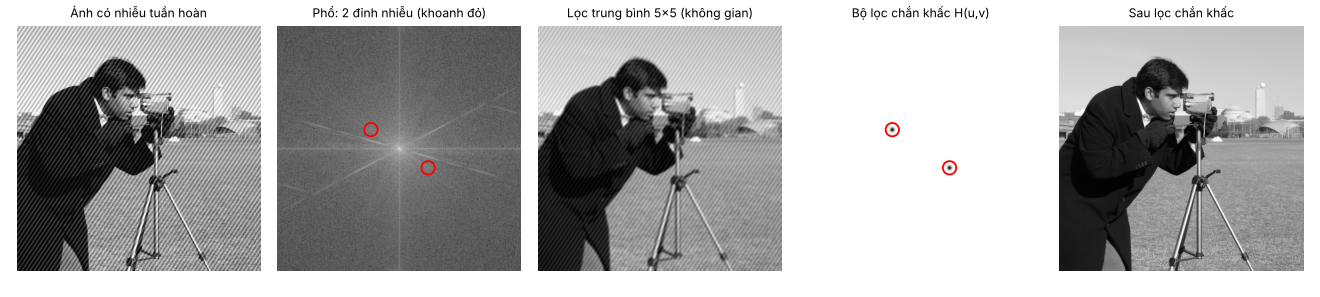
\includegraphics[width=\textwidth]{w7_periodic.png}
\caption{Nhiễu tuần hoàn: trong miền không gian phủ khắp ảnh, trong miền tần số chỉ là hai đỉnh (khoanh đỏ). Bộ lọc chắn khấc đặt $H = 0$ tại hai đỉnh đó.}
\label{fig:w7_periodic}
\end{figure}

% =====================================================================
\subsection{Khái niệm tần số trong ảnh}
\label{subsec:w7_frequency}

\textit{Câu hỏi: Giải thích khái niệm tần số (tần số không gian) trong ảnh.}

\textbf{Tần số một chiều.} Với tín hiệu theo thời gian, tần số là số dao động trong một đơn vị thời gian. Trong ảnh, biến số là \emph{vị trí}, nên tần số không gian là \emph{số chu kỳ biến thiên mức xám trên một đơn vị độ dài} (chu kỳ/điểm ảnh, hoặc số chu kỳ trên toàn bề rộng ảnh). Bài giảng (trang 3--5) mô tả một hàm sin bởi chu kỳ $L$, tần số $1/L$, biên độ $A$, pha $\phi$, và hiển thị nó thành ảnh
\begin{equation}
f(x, y) = 128 + A\sin\!\left(\frac{2\pi u x}{N - 1} + \phi\right),
\end{equation}
trong đó $u$ là số chu kỳ trên bề rộng ảnh: $u$ càng lớn thì các sọc sáng tối càng dày (trang 6: $u = 3$ và $u = 6$); $A$ là độ tương phản của sọc; $\phi$ làm các sọc dịch chuyển.

\textbf{Tần số hai chiều.} Thành phần $\sin\big(2\pi(ux/M + vy/N)\big)$ là các sọc song song có:
\begin{itemize}
    \item \emph{hướng}: vector $(u, v)$ vuông góc với các sọc (trang 7: $u = 0, v = 4$ cho sọc ngang; $u = 3, v = 5$ cho sọc xiên);
    \item \emph{độ dày}: khoảng cách giữa hai sọc (bước sóng) tỉ lệ nghịch với $\sqrt{(u/M)^2 + (v/N)^2}$, tức với khoảng cách từ $(u, v)$ tới gốc của mặt phẳng tần số.
\end{itemize}
Hình~\ref{fig:w7_sinusoids} cho thấy mỗi ảnh sin chỉ tạo \emph{hai điểm} đối xứng qua tâm trên phổ biên độ, nằm theo hướng $(u, v)$ và cách tâm một khoảng tỉ lệ với tần số.

\begin{figure}[ht]
\centering
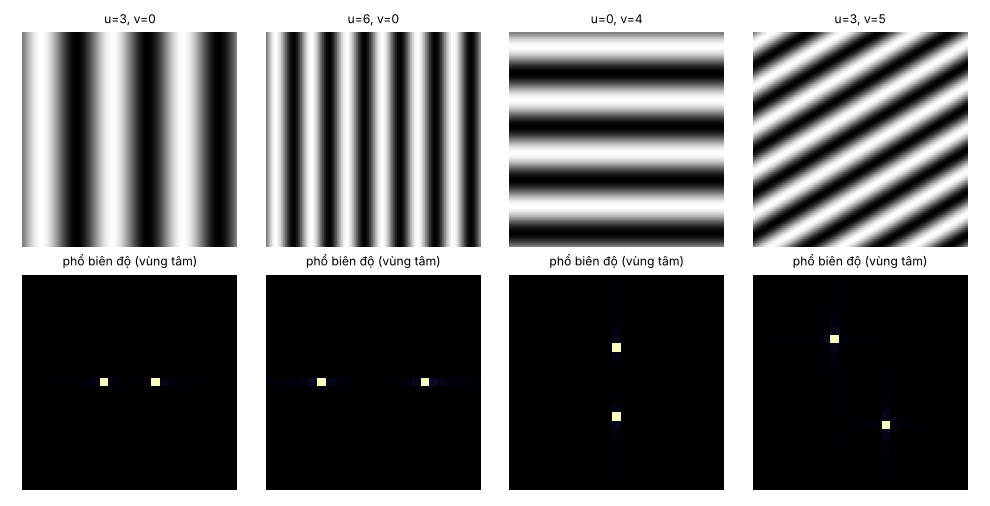
\includegraphics[width=0.9\textwidth]{w7_sinusoids.png}
\caption{Ảnh sin với các tần số $(u, v)$ khác nhau (hàng trên) và phổ biên độ (hàng dưới, vùng $25 \times 25$ quanh tâm).}
\label{fig:w7_sinusoids}
\end{figure}

\textbf{Tần số trong một ảnh bất kỳ.} Theo~(\ref{eq:w7_dft}), mọi ảnh là tổng có trọng số của các ảnh sin cơ sở (trang 12). Hệ số $F(u, v)$ cho biết ảnh ``chứa'' bao nhiêu thành phần sọc có tần số và hướng $(u, v)$: biên độ $|F|$ là độ mạnh, pha $\phi$ là vị trí của sọc. Do đó:
\begin{itemize}
    \item \textbf{Tần số $0$} (thành phần một chiều, DC): $F(0, 0) = \frac{1}{MN}\sum f$ là độ sáng trung bình (trang 18).
    \item \textbf{Tần số thấp}: các biến thiên chậm, trên khoảng cách lớn — vùng đồng nhất, sự thay đổi độ sáng dần dần, hình dạng tổng thể.
    \item \textbf{Tần số cao}: các biến thiên nhanh, trên khoảng cách vài điểm ảnh — biên cạnh, chi tiết nhỏ, kết cấu mịn, và nhiễu. Biên càng sắc thì phổ càng trải rộng ra tần số cao (trang 20: biên sắc so với biên mờ).
    \item Tần số cao nhất biểu diễn được là $\frac{1}{2}$ chu kỳ/điểm ảnh (sáng, tối xen kẽ từng điểm), theo định lý lấy mẫu Nyquist.
\end{itemize}
Các biên thẳng trong ảnh tạo ra các vệt sáng trên phổ \emph{vuông góc} với biên (vệt ngang và dọc rõ nét trên phổ của ảnh \texttt{camera} ở Hình~\ref{fig:w7_periodic}, phần lớn do sự gián đoạn giữa hai cạnh đối diện của ảnh khi DFT coi ảnh là tuần hoàn). Pha mang phần lớn thông tin cấu trúc: ghép biên độ của ảnh này với pha của ảnh kia, kết quả trông giống ảnh cung cấp pha~\citep{oppenheim1981importance}.

% =====================================================================
\subsection{Phân biệt chuỗi Fourier và phép biến đổi Fourier}
\label{subsec:w7_series_vs_transform}

\textit{Câu hỏi: Phân biệt chuỗi Fourier (Fourier series, Bài giảng 7, trang 8--12) và phép biến đổi Fourier (Fourier transform, trang 13--14).}

\textbf{Chuỗi Fourier} áp dụng cho hàm \emph{tuần hoàn} chu kỳ $L$: hàm được biểu diễn thành tổng (đếm được) các sóng sin có tần số là \emph{bội nguyên} $n/L$ của tần số cơ bản (trang 8):
\begin{equation}
f(x) = a_0 + \sum_{n=1}^{\infty}\left[a_n\cos\frac{2\pi n x}{L} + b_n\sin\frac{2\pi n x}{L}\right],
\end{equation}
dạng phức tương đương $f(x) = \sum_{n=-\infty}^{\infty} c_n e^{2\pi i n x/L}$ với
\begin{equation}
c_n = \frac{1}{L}\int_0^L f(x)\,e^{-2\pi i n x / L}\,dx.
\end{equation}
Hình 7.1 ở trang 9 minh họa: cộng dần $1$, $3$, $15$ số hạng sin, tổng tiến dần tới sóng vuông.

\textbf{Biến đổi Fourier} áp dụng cho hàm \emph{không tuần hoàn} (khả tích trên toàn trục): hàm được biểu diễn bằng tích phân trên một \emph{dải tần số liên tục} (trang 13):
\begin{equation}
F(u) = \int_{-\infty}^{\infty} f(x)\,e^{-2\pi i u x}\,dx, \qquad f(x) = \int_{-\infty}^{\infty} F(u)\,e^{2\pi i u x}\,du.
\end{equation}

\textbf{Mối liên hệ.} Có thể xem một hàm không tuần hoàn là hàm tuần hoàn với chu kỳ $L \to \infty$. Khi $L$ tăng, khoảng cách giữa hai tần số liền kề $\Delta u = 1/L$ giảm dần về $0$: các vạch phổ rời rạc $c_n$ dày lên thành một hàm liên tục, $L c_n \to F(n/L)$, và tổng $\sum_n$ trở thành tích phân $\int du$. Ngược lại, chuỗi Fourier của hàm tuần hoàn chính là biến đổi Fourier của nó khi cho phép hàm xung Dirac (phổ chỉ khác $0$ tại các tần số $n/L$).

\textbf{DFT dùng cho ảnh số} thực chất là một chuỗi Fourier \emph{hữu hạn}: ảnh có hữu hạn mẫu $M \times N$ nên chỉ có hữu hạn tần số $u = 0, \ldots, M - 1$, và DFT ngầm coi ảnh là \emph{một chu kỳ} của một ảnh tuần hoàn vô hạn. Vì vậy DFT thừa hưởng cả hai: tính rời rạc tần số của chuỗi Fourier (do ảnh hữu hạn/tuần hoàn) và tính tuần hoàn phổ của tín hiệu lấy mẫu.

\begin{table}[ht]
\centering
\scriptsize
\caption{Chuỗi Fourier, biến đổi Fourier và DFT}
\label{tab:w7_series_transform}
\renewcommand{\arraystretch}{1.3}
\begin{tabularx}{\textwidth}{|p{2.2cm}|X|X|X|}
\hline
\textbf{Tiêu chí} & \textbf{Chuỗi Fourier} & \textbf{Biến đổi Fourier} & \textbf{DFT (ảnh số)} \\
\hline
Hàm áp dụng & Liên tục, tuần hoàn chu kỳ $L$ & Liên tục, không tuần hoàn, khả tích & Rời rạc, hữu hạn $M \times N$ mẫu (coi như tuần hoàn) \\
\hline
Tần số & Rời rạc, bội nguyên $n/L$, vô hạn đếm được & Liên tục trên toàn trục $\mathbb{R}$ & Rời rạc, hữu hạn: $u = 0, \ldots, M - 1$ \\
\hline
Biểu diễn & Tổng vô hạn $\sum_n$ & Tích phân $\int du$ & Tổng hữu hạn, tính được chính xác \\
\hline
Kết quả & Dãy hệ số $a_n, b_n$ (hoặc $c_n$) & Hàm phổ $F(u)$ liên tục & Mảng $F(u, v)$ cùng kích thước ảnh \\
\hline
Vai trò & Nền tảng lý thuyết: ``mọi hàm tuần hoàn là tổng các sin'' & Công cụ phân tích: định lý tích chập, thiết kế bộ lọc & Công cụ tính toán thực tế, có giải thuật FFT $O(MN\log MN)$ \\
\hline
\end{tabularx}
\end{table}

% =====================================================================
\subsection{Ý nghĩa và ứng dụng của định lý tích chập}
\label{subsec:w7_conv_theorem}

\textit{Câu hỏi: Trang 15 của Bài giảng 7 phát biểu định lý tích chập: $\zeta\{(f * h)(x, y)\} = F(u, v)\,H(u, v)$ và $\zeta\{f(x, y)\,h(x, y)\} = (F * H)(u, v)$. Giải thích ý nghĩa và nêu ứng dụng của định lý này.}

\textbf{Phát biểu thứ nhất: tích chập trong miền không gian tương ứng với phép nhân trong miền tần số.} Với quy ước chuẩn hóa của bài giảng (trang 16 và trang 26: $f * h = \frac{1}{MN}\sum_{m}\sum_{n} f(x - m, y - n)\,h(m, n)$, chỉ số lấy theo modulo $M$, $N$):
\begin{equation}
\zeta\{f * h\}(u, v) = F(u, v)\,H(u, v).
\end{equation}
\emph{Chứng minh} (một chiều, hai chiều tương tự): đặt $x' = x - m$,
\begin{align*}
\frac{1}{M}\sum_{x}\Big[\frac{1}{M}\sum_{m} f(x - m)h(m)\Big]e^{-2\pi i u x/M}
&= \Big[\frac{1}{M}\sum_{m} h(m)e^{-2\pi i u m/M}\Big]\\
&\quad \times \Big[\frac{1}{M}\sum_{x'} f(x')e^{-2\pi i u x'/M}\Big] = H(u)F(u),
\end{align*}
vì $e^{-2\pi i u x/M} = e^{-2\pi i u m/M}e^{-2\pi i u x'/M}$ và tổng theo $x'$ chạy hết một chu kỳ. Nhóm đã kiểm tra bằng số trên ảnh \texttt{camera}: tích chập vòng trực tiếp và $\zeta^{-1}\{F \cdot H\}$ sai khác tối đa $1{,}7 \times 10^{-13}$.

\textbf{Ý nghĩa.}
\begin{enumerate}
    \item \textbf{Bộ lọc tuyến tính bất biến dịch chuyển tác động độc lập lên từng tần số.} Thành phần sin tần số $(u, v)$ của ảnh đi qua bộ lọc vẫn là sin cùng tần số, chỉ bị nhân biên độ với $|H(u, v)|$ và dịch pha một lượng $\arg H(u, v)$. Mọi bộ lọc tuyến tính (trung bình, Gauss, Sobel, Laplace ở Tuần 6) đều được mô tả trọn vẹn bằng một hàm $H(u, v)$ — ``đáp ứng tần số'' của nó.
    \item \textbf{Một phép toán phức tạp ($O(k^2)$ phép nhân mỗi điểm) trở thành một phép nhân đơn giản} ($1$ phép nhân mỗi tần số).
\end{enumerate}

\textbf{Ứng dụng.}
\begin{itemize}
    \item \textbf{Lọc nhanh}: $f * h = \zeta^{-1}\{\zeta\{f\}\cdot\zeta\{h\}\}$ bằng FFT, hiệu quả với mặt nạ lớn (Bảng~\ref{tab:w7_timing}). Cần đệm $0$ (hoặc phản xạ) để kích thước $\ge M + k - 1$, vì DFT cho tích chập \emph{vòng}.
    \item \textbf{Lọc trong miền tần số}: thiết kế trực tiếp $H(u, v)$ (lọc thông thấp, thông cao, chắn dải, chắn khấc) — toàn bộ mục 7.4 của bài giảng (trang 26--51) dựa trên định lý này.
    \item \textbf{Phân tích bộ lọc không gian}: giải thích vì sao lọc trung bình để lọt một phần tần số cao (biến đổi Fourier của hàm hộp là hàm sinc có các thùy phụ), còn lọc Gauss thì không (biến đổi Fourier của Gauss là Gauss).
    \item \textbf{Khôi phục ảnh}: ảnh mờ $g = f * h + n$ có $G = FH + N$; lọc ngược $\hat F = G/H$, lọc Wiener $\hat F = \frac{H^*}{|H|^2 + K}G$.
    \item \textbf{So khớp mẫu}: tương quan chéo giữa ảnh và mẫu (một dạng tích chập) tính nhanh bằng $F \cdot T^*$; đăng ký ảnh bằng tương quan pha.
    \item \textbf{Học sâu}: một số thư viện tính lớp tích chập với nhân lớn bằng FFT.
\end{itemize}

% =====================================================================
\subsection{Ý nghĩa của phát biểu thứ hai trong định lý tích chập}
\label{subsec:w7_theorem2}

\textit{Câu hỏi: Phát biểu thứ hai của định lý tích chập (trang 15), $\zeta\{f(x, y)\,h(x, y)\} = (F * H)(u, v)$, dùng để làm gì?}

Phát biểu thứ hai là đối ngẫu của phát biểu thứ nhất: \emph{nhân hai hàm trong miền không gian tương ứng với tích chập phổ của chúng trong miền tần số}. Chứng minh tương tự (vai trò của $x$ và $u$ đổi chỗ cho nhau). Phép nhân điểm theo điểm xuất hiện rất thường xuyên trong xử lý ảnh, và phát biểu này cho biết phép nhân đó ``làm gì'' với phổ:

\begin{enumerate}
    \item \textbf{Dịch phổ về tâm.} Nhân ảnh với $e^{2\pi i(u_0 x/M + v_0 y/N)}$ (phổ là một xung tại $(u_0, v_0)$) thì phổ bị dịch: $\zeta\{f\,e^{2\pi i(u_0 x/M + v_0 y/N)}\} = F(u - u_0, v - v_0)$. Với $u_0 = M/2$, $v_0 = N/2$, thừa số này chính là $(-1)^{x + y}$:
    \begin{equation}
    \zeta\{f(x, y)(-1)^{x + y}\} = F(u - M/2,\ v - N/2).
    \end{equation}
    Đây là lý do các hình phổ trong bài giảng có tần số $0$ ở giữa, và các bộ lọc ở trang 32--51 dùng $D(u, v) = \big[(u - M/2)^2 + (v - N/2)^2\big]^{1/2}$ (khoảng cách tới tâm phổ).
    \item \textbf{Cắt ảnh và cửa sổ hóa.} Ảnh hữu hạn là ảnh vô hạn nhân với một cửa sổ chữ nhật; phổ thu được là phổ thật tích chập với hàm sinc 2 chiều. Hệ quả là phổ bị ``rò rỉ'' (leakage) và xuất hiện các vệt ngang dọc qua tâm phổ (thấy rõ trong phổ ở trang 17, 22 và Hình~\ref{fig:w7_periodic}). Nhân ảnh với cửa sổ mềm (Hann, Gauss) trước khi biến đổi làm giảm hiện tượng này.
    \item \textbf{Lấy mẫu và chồng phổ.} Lấy mẫu ảnh liên tục là nhân với một lưới xung; phổ của lưới xung cũng là lưới xung, nên phổ ảnh số là phổ ảnh liên tục được \emph{lặp lại tuần hoàn}. Nếu lấy mẫu thưa, các bản lặp chồng lên nhau gây răng cưa (aliasing). Từ đây suy ra định lý lấy mẫu Nyquist và lý do phải lọc thông thấp trước khi thu nhỏ ảnh (Mục~\ref{subsec:w6_geo_difficulty}).
    \item \textbf{Điều chế.} Nhân với $\cos(2\pi u_0 x)$ tách phổ thành hai bản dịch về $\pm u_0$; đây là cơ chế sinh ra nhiễu tuần hoàn và hiện tượng moiré khi hai mẫu sọc chồng lên nhau.
    \item \textbf{Mô hình chiếu sáng -- phản xạ.} Ảnh $f = i \cdot r$ (độ chiếu sáng nhân với hệ số phản xạ) có phổ là tích chập của hai phổ, nên không thể tách bằng một bộ lọc tuyến tính. Lấy logarit đưa tích thành tổng, $\ln f = \ln i + \ln r$, rồi mới lọc — đây là lọc đồng hình (homomorphic filtering).
    \item \textbf{Phân tích tác động của mặt nạ, trọng số không gian} như vignetting của ống kính, hay tác động của việc đặt $0$ cho một vùng ảnh, lên phổ của ảnh.
\end{enumerate}

% =====================================================================
\subsection{Xác định hàm truyền \texorpdfstring{$H(u, v)$}{H(u, v)} khi làm trơn ảnh trong miền tần số}
\label{subsec:w7_find_H}

\textit{Câu hỏi: Khi làm trơn ảnh trong miền tần số, hàm truyền $H(u, v)$ được xác định như thế nào?}

\textbf{Yêu cầu đối với $H$.} Làm trơn là giữ lại tần số thấp (vùng đồng nhất, hình dạng tổng thể) và làm suy giảm tần số cao (chi tiết, nhiễu). Vì vậy $H$ là bộ lọc \emph{thông thấp} thỏa:
\begin{enumerate}
    \item $H(0, 0) = 1$ (sau khi dịch tâm: $H$ tại tâm bằng $1$), để độ sáng trung bình không đổi;
    \item $0 \le H \le 1$ và $H$ \emph{giảm dần} khi khoảng cách $D(u, v)$ tới tâm tăng;
    \item $H$ là hàm \emph{thực}, \emph{đối xứng}: $H(u, v) = H(-u, -v)$, để không làm lệch pha (bộ lọc ``pha không''), ảnh kết quả không bị dịch chuyển và vẫn là số thực;
    \item thường chọn $H$ \emph{đối xứng tròn}, chỉ phụ thuộc $D(u, v)$, để làm trơn như nhau theo mọi hướng.
\end{enumerate}

\textbf{Các dạng $H$ thường dùng} (trang 31--40), với $D_0$ là tần số cắt:
\begin{equation}
H_{\text{lý tưởng}} = \begin{cases} 1, & D \le D_0 \\ 0, & D > D_0 \end{cases}, \qquad
H_{\text{Butterworth}} = \frac{1}{1 + (D/D_0)^{2n}}, \qquad
H_{\text{Gauss}} = e^{-D^2/2D_0^2}.
\end{equation}
Bài giảng viết bộ lọc Gauss với $\sigma$ (trang 38); đặt $\sigma = D_0$ để thống nhất ký hiệu.

\textbf{Cách khác: lấy $H$ từ một bộ lọc không gian.} Nếu đã có mặt nạ không gian $h$ (ví dụ trung bình $3 \times 3$, Gauss $5 \times 5$), đặt $h$ vào một mảng $0$ cùng kích thước ảnh đã đệm (tâm mặt nạ ở gốc tọa độ) rồi tính $H = \zeta\{h\}$. Theo định lý tích chập, kết quả lọc giống hệt lọc trong miền không gian.

\textbf{Chọn tần số cắt $D_0$.} $D_0$ quyết định mức độ làm trơn. Một cách chọn khách quan là theo tỉ lệ năng lượng giữ lại~\citep{gonzalez2018digital}:
\begin{equation}
\alpha(D_0) = 100 \cdot \frac{\sum_{D(u, v) \le D_0} |F(u, v)|^2}{\sum_{u, v}|F(u, v)|^2}\ (\%).
\end{equation}
Với ảnh \texttt{camera}: $\alpha = 96{,}8\%$ ($D_0 = 10$), $98{,}5\%$ ($D_0 = 30$), $99{,}2\%$ ($D_0 = 60$), $99{,}7\%$ ($D_0 = 120$). Phần năng lượng nhỏ ở tần số cao lại chứa toàn bộ chi tiết, nên $1$--$2\%$ năng lượng bị loại cũng đủ làm ảnh mờ rõ rệt (Hình~\ref{fig:w7_ilpf}). Có thể chọn $D_0$ theo kích thước chi tiết muốn xóa: chi tiết có bước sóng $\lambda$ điểm ảnh tương ứng với $D \approx M/\lambda$.

\textbf{Quy trình lọc} (sơ đồ ở trang 27; Giải thuật~\ref{alg:w7_filter}).

\begin{algorithm}[ht]
\caption{Lọc ảnh trong miền tần số}
\label{alg:w7_filter}
\begin{algorithmic}[1]
\Require Ảnh $f$ kích thước $M \times N$; hàm $H(D)$ (ví dụ thông thấp với tham số $D_0$)
\Ensure Ảnh đã lọc $g$
\State Đệm $f$ thành ảnh $f_p$ kích thước $P \times Q = 2M \times 2N$ (đệm $0$ hoặc phản xạ biên) \Comment{tránh quấn của tích chập vòng}
\State $f_p(x, y) \gets f_p(x, y)\,(-1)^{x + y}$ \Comment{dịch tâm phổ (Mục~\ref{subsec:w7_theorem2})}
\State $F \gets \mathrm{FFT}(f_p)$
\For{mỗi $(u, v)$} \State $D \gets \sqrt{(u - P/2)^2 + (v - Q/2)^2}$; \quad $G(u, v) \gets H(D)\,F(u, v)$ \EndFor
\State $g_p \gets \mathrm{Re}\{\mathrm{IFFT}(G)\}\,(-1)^{x + y}$ \Comment{bỏ phần ảo do sai số làm tròn}
\State $g \gets$ vùng $M \times N$ của $g_p$ tương ứng với ảnh gốc
\State \Return $g$
\end{algorithmic}
\end{algorithm}

% =====================================================================
\subsection{Cơ chế hoạt động của bộ lọc thông thấp lý tưởng; ảnh hưởng của \texorpdfstring{$D_0$}{D0}}
\label{subsec:w7_ilpf}

\textit{Câu hỏi: Trang 32 của Bài giảng 7 định nghĩa bộ lọc thông thấp lý tưởng (ILPF): $H(u, v) = 1$ nếu $D(u, v) \le D_0$ và $H(u, v) = 0$ nếu $D(u, v) > D_0$, với $D(u, v) = \big[(u - M/2)^2 + (v - N/2)^2\big]^{1/2}$. Giải thích cơ chế hoạt động của bộ lọc này. Điều gì xảy ra khi $D_0$ lớn hoặc nhỏ?}

\textbf{Cơ chế.} Trên mặt phẳng tần số đã dịch tâm, $H$ là một \emph{hình tròn} bán kính $D_0$ (hình trụ ở trang 33): mọi thành phần tần số nằm trong đường tròn được giữ \emph{nguyên vẹn} ($H = 1$), mọi thành phần nằm ngoài bị \emph{xóa hoàn toàn} ($H = 0$), không có vùng chuyển tiếp. Ảnh ra $g = \zeta^{-1}\{H F\}$ chỉ còn các biến thiên có bước sóng lớn hơn khoảng $M/D_0$ điểm ảnh, nên các chi tiết nhỏ hơn bị xóa và ảnh bị làm trơn.

\textbf{Hiện tượng gợn sóng (ringing).} Theo định lý tích chập, lọc bằng $H$ tương đương với tích chập ảnh với nhân không gian $h = \zeta^{-1}\{H\}$. Biến đổi ngược của một hình tròn là hàm $\frac{J_1(r)}{r}$ (hàm Bessel bậc một, ``sinc tròn''): một đỉnh chính ở tâm bao quanh bởi các vòng tròn \emph{dương âm xen kẽ} giảm dần (Hình~\ref{fig:w7_profiles}, phải: thùy âm thứ nhất sâu tới $-13{,}6\%$ đỉnh chính). Tích chập với nhân có thùy âm làm xuất hiện các gợn sóng song song chạy dọc theo mọi biên cạnh — hiện tượng Gibbs, thấy rõ trong các ảnh ở trang 34 và Hình~\ref{fig:w7_ilpf}. Nguyên nhân sâu xa là $H$ có bước nhảy đột ngột từ $1$ xuống $0$.

\textbf{Ảnh hưởng của $D_0$.} Bán kính đỉnh chính của $h$ tỉ lệ nghịch với $D_0$ (tính chất co giãn của biến đổi Fourier).
\begin{itemize}
    \item \textbf{$D_0$ nhỏ}: giữ rất ít tần số. Nhân $h$ rộng nên ảnh rất mờ, chỉ còn hình dạng thô; các vòng gợn sóng rộng và nổi rõ. Với ảnh \texttt{camera}, $D_0 = 10$ chỉ giữ $96{,}8\%$ năng lượng và ảnh gần như không còn nhận ra chi tiết.
    \item \textbf{$D_0$ tăng}: giữ được nhiều tần số hơn, ảnh bớt mờ; gợn sóng mảnh hơn và nằm sát biên hơn nhưng vẫn còn ($D_0 = 30$, $60$).
    \item \textbf{$D_0$ lớn}: hầu hết phổ được giữ lại, ảnh gần như ảnh gốc, tác dụng làm trơn và khử nhiễu rất ít ($D_0 = 120$: $99{,}7\%$ năng lượng). Khi $D_0 \ge \sqrt{(M/2)^2 + (N/2)^2}$, $H \equiv 1$ và ảnh không đổi.
\end{itemize}

\begin{figure}[ht]
\centering
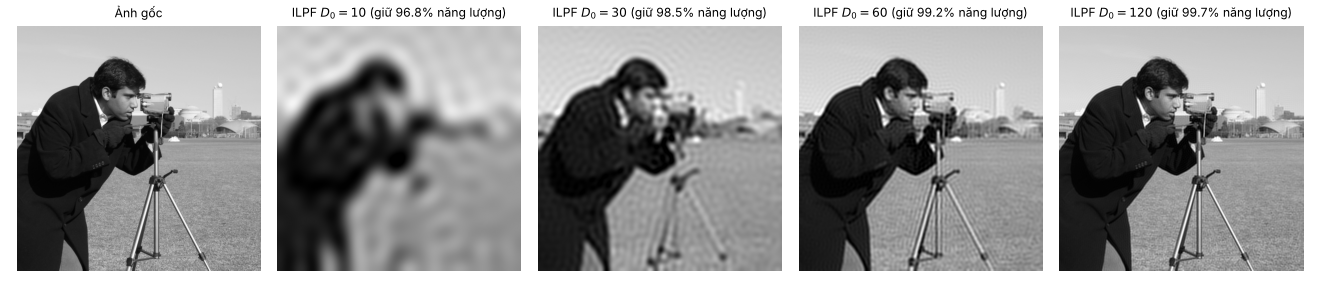
\includegraphics[width=\textwidth]{w7_ilpf.png}
\caption{Lọc thông thấp lý tưởng với $D_0 = 10, 30, 60, 120$. Gợn sóng thấy rõ quanh người và chân máy ảnh.}
\label{fig:w7_ilpf}
\end{figure}

\textbf{Nhận xét.} ILPF ``lý tưởng'' về mặt định nghĩa nhưng không lý tưởng về chất lượng: hiện tượng gợn sóng khiến nó ít được dùng trong thực tế. ILPF không thể chế tạo bằng mạch điện tử, nhưng cài đặt được trên máy tính; giá trị của nó là để minh họa khái niệm tần số cắt và hiện tượng gợn sóng.

% =====================================================================
\subsection{Quá trình hoạt động của bộ lọc thông thấp Butterworth}
\label{subsec:w7_blpf}

\textit{Câu hỏi: Giải thích quá trình hoạt động của bộ lọc thông thấp Butterworth (BLPF, trang 35--37) $H(u, v) = \dfrac{1}{1 + \big[D(u, v)/D_0\big]^{2n}}$.}

\textbf{Quá trình lọc} theo Giải thuật~\ref{alg:w7_filter}: biến đổi ảnh sang miền tần số, nhân mỗi hệ số $F(u, v)$ với $H$ tính theo khoảng cách $D(u, v)$ tới tâm phổ, rồi biến đổi ngược. Khác với ILPF, BLPF \emph{giảm dần} hệ số theo tần số chứ không cắt đột ngột:
\begin{itemize}
    \item $D = 0$: $H = 1$, thành phần trung bình được giữ nguyên.
    \item $D \ll D_0$: $(D/D_0)^{2n} \approx 0$, $H \approx 1$, tần số thấp đi qua gần như nguyên vẹn. Vùng này rất phẳng: $H$ có $2n - 1$ đạo hàm đầu bằng $0$ tại $D = 0$ (tính chất ``phẳng tối đa'' của Butterworth).
    \item $D = D_0$: $H = 0{,}5$ với mọi $n$. $D_0$ là điểm mà biên độ giảm còn một nửa.
    \item $D \gg D_0$: $H \approx (D_0/D)^{2n}$, tần số cao bị suy giảm theo hàm lũy thừa; tăng gấp đôi tần số thì $H$ giảm $2^{2n}$ lần.
\end{itemize}

\textbf{Vai trò của bậc $n$.} $n$ điều khiển \emph{độ dốc} của vùng chuyển tiếp quanh $D_0$ (Hình~\ref{fig:w7_profiles}, trái):
\begin{itemize}
    \item $n = 1$: chuyển tiếp rất thoải, nhân không gian dương hoàn toàn, \emph{không có gợn sóng}, nhưng lọt khá nhiều tần số cao ($H = 0{,}04$ tại $D = 5D_0$).
    \item $n = 2$: cân bằng tốt giữa độ sắc của tần số cắt và gợn sóng; thùy âm của nhân không gian chỉ khoảng $-1{,}4\%$, gợn sóng hầu như không thấy được. Đây là lựa chọn thường dùng nhất.
    \item $n$ lớn ($n = 5$: thùy âm $-8{,}6\%$; $n = 20$): chuyển tiếp ngày càng dốc, BLPF tiến dần tới ILPF và gợn sóng xuất hiện rõ (Hình~\ref{fig:w7_lp_compare}).
\end{itemize}
Như vậy BLPF là một \emph{họ} bộ lọc nối liền giữa bộ lọc rất mềm (gần Gauss khi $n$ nhỏ) và bộ lọc lý tưởng ($n \to \infty$), cho phép chọn điểm cân bằng giữa độ sắc của tần số cắt và hiện tượng gợn sóng.

\begin{figure}[ht]
\centering
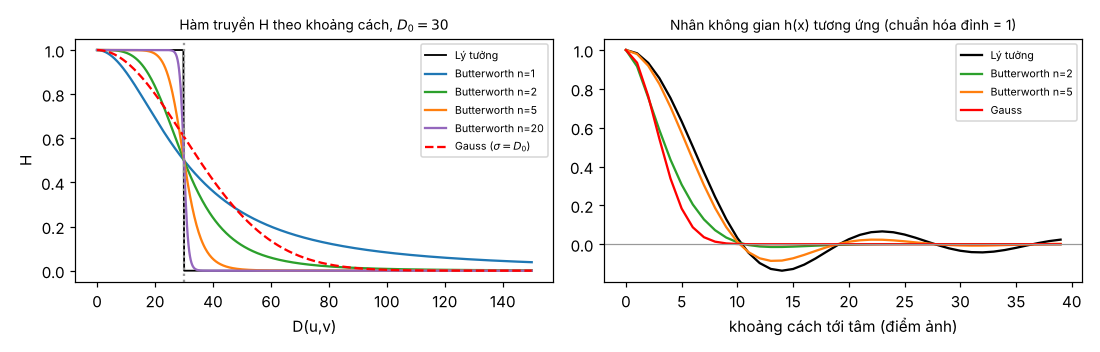
\includegraphics[width=\textwidth]{w7_profiles.png}
\caption{Trái: hàm truyền $H(D)$ của bộ lọc lý tưởng, Butterworth bậc $1, 2, 5, 20$ và Gauss với $D_0 = 30$. Phải: lát cắt qua tâm của nhân không gian $h = \zeta^{-1}\{H\}$; thùy âm là nguyên nhân gây gợn sóng.}
\label{fig:w7_profiles}
\end{figure}

% =====================================================================
\subsection{So sánh bộ lọc thông thấp Gauss và Butterworth}
\label{subsec:w7_gauss_vs_butter}

\textit{Câu hỏi: So sánh hai bộ lọc thông thấp Gauss (GLPF, trang 38--40) và Butterworth (BLPF, trang 35--37).}

\begin{table}[ht]
\centering
\scriptsize
\caption{So sánh bộ lọc thông thấp Gauss và Butterworth}
\label{tab:w7_glpf_blpf}
\renewcommand{\arraystretch}{1.3}
\begin{tabularx}{\textwidth}{|p{2.3cm}|X|X|}
\hline
\textbf{Tiêu chí} & \textbf{Gauss (GLPF)} & \textbf{Butterworth (BLPF)} \\
\hline
Hàm truyền & $H = e^{-D^2/2D_0^2}$ & $H = 1/\big(1 + (D/D_0)^{2n}\big)$ \\
\hline
Tham số & Một tham số $D_0$ ($\sigma$) & Hai tham số $D_0$, $n$ \\
\hline
Giá trị tại $D = D_0$ & $e^{-1/2} \approx 0{,}607$ & $0{,}5$ (với mọi $n$) \\
\hline
Độ dốc chuyển tiếp & Cố định, khá thoải & Điều chỉnh được qua $n$; từ rất thoải ($n = 1$) tới gần như cắt đột ngột ($n$ lớn) \\
\hline
Suy giảm ở tần số cao & Rất nhanh (hàm mũ của $D^2$) & Theo lũy thừa $(D_0/D)^{2n}$, chậm hơn khi $n$ nhỏ \\
\hline
Nhân không gian $h$ & Cũng là Gauss: luôn dương, không có thùy âm & Có thùy âm khi $n \ge 2$, càng sâu khi $n$ càng lớn \\
\hline
Gợn sóng & Không bao giờ có & Không có ($n = 1$), không đáng kể ($n = 2$), rõ ($n \ge 5$) \\
\hline
Tách được, cài đặt trong miền không gian & Có ($e^{-(u^2 + v^2)} = e^{-u^2}e^{-v^2}$); dễ cài bằng mặt nạ Gauss tách được & Không tách được; nhân không gian không có dạng đóng đơn giản, thường cài trong miền tần số \\
\hline
Bộ lọc thông cao tương ứng & $1 - H_{\text{Gauss}}$ (trang 48) & $1/\big(1 + (D_0/D)^{2n}\big)$ (trang 45) \\
\hline
Ưu điểm & Không có gợn sóng; dễ phân tích (cặp Fourier Gauss -- Gauss); tương ứng trực tiếp với lọc Gauss Tuần 6 & Linh hoạt; tần số cắt sắc hơn nên giữ chi tiết dưới $D_0$ tốt hơn với cùng mức xóa tần số cao \\
\hline
Nhược điểm & Không điều chỉnh được độ sắc của tần số cắt; để xóa nhiều tần số cao phải chấp nhận làm suy giảm cả tần số trung bình & Thêm một tham số cần chọn; $n$ lớn gây gợn sóng \\
\hline
Thực nghiệm ($D_0 = 30$, Hình~\ref{fig:w7_lp_compare}) & Ảnh mờ đều, không gợn; PSNR so với ảnh gốc $24{,}56$ dB & $n = 2$: $23{,}96$ dB, không thấy gợn; $n = 5$: $23{,}48$ dB, có gợn quanh biên \\
\hline
\end{tabularx}
\end{table}

Ở Bảng~\ref{tab:w7_glpf_blpf}, PSNR so với \emph{ảnh gốc} chỉ đo mức thay đổi do lọc gây ra: cùng $D_0$, GLPF có $H(D_0) = 0{,}61 > 0{,}5$ nên giữ lại nhiều năng lượng hơn và ít làm mờ hơn một chút; không nên hiểu đây là ``chất lượng tốt hơn''. Khi cần mức làm trơn tương đương, có thể chọn $D_0$ của hai bộ lọc khác nhau.

\begin{figure}[ht]
\centering
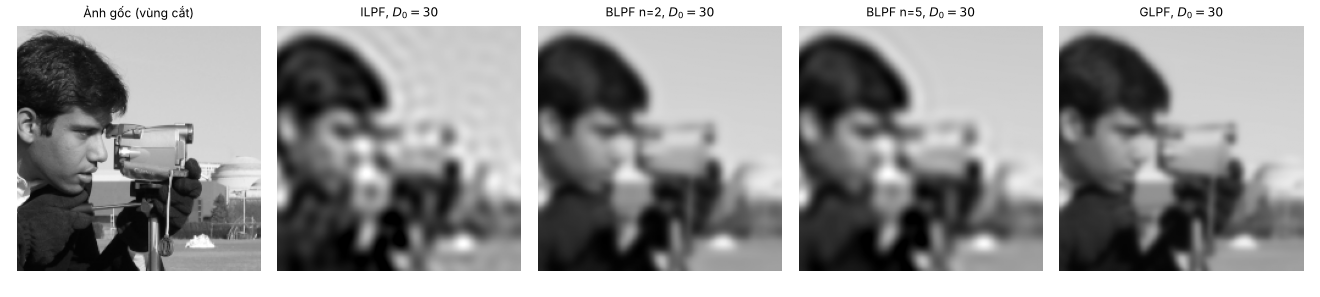
\includegraphics[width=\textwidth]{w7_lp_compare.png}
\caption{Bộ lọc lý tưởng, Butterworth bậc $2$, bậc $5$ và Gauss cùng $D_0 = 30$ (vùng cắt). Gợn sóng rõ ở ILPF, thấy được ở BLPF bậc $5$, không có ở BLPF bậc $2$ và GLPF.}
\label{fig:w7_lp_compare}
\end{figure}

\textbf{Kết luận.} Hai bộ lọc rất gần nhau khi $n = 2$. GLPF được ưu tiên khi tuyệt đối không được có gợn sóng (ảnh y khoa, tiền xử lý cho phát hiện biên) hoặc khi muốn cài đặt trong miền không gian; BLPF được ưu tiên khi cần kiểm soát độ sắc của tần số cắt.

% =====================================================================
\subsection{Giá trị thông tin tại mỗi điểm của ảnh kết quả phát hiện biên trong miền không gian và miền tần số}
\label{subsec:w7_edge_info}

\textit{Câu hỏi: Với ảnh kết quả của phép phát hiện biên cạnh, giá trị tại mỗi điểm trong miền không gian và giá trị tại mỗi điểm trong miền tần số của ảnh đó mang thông tin gì?}

Gọi $e(x, y)$ là ảnh kết quả phát hiện biên — ví dụ đầu ra của bộ lọc thông cao, của Laplace (Tuần 6), hay độ lớn gradient — và $E(u, v) = \zeta\{e\}$.

\textbf{Trong miền không gian}, giá trị $e(x, y)$ là thông tin \emph{cục bộ}, gắn với vị trí $(x, y)$:
\begin{itemize}
    \item với độ lớn gradient: \emph{độ mạnh} của biên tại đúng điểm đó, tức tốc độ thay đổi mức xám (kèm theo hướng $\phi(x, y)$ nếu lưu thêm);
    \item với Laplace hay bộ lọc thông cao: giá trị có dấu, gần $0$ trong vùng đồng nhất, lớn ở hai bên biên, dấu cho biết điểm nằm ở phía sáng hay phía tối, điểm qua $0$ là tâm biên;
    \item sau phân ngưỡng: điểm này có thuộc biên hay không ($0$/$1$).
\end{itemize}
Nói ngắn gọn: miền không gian cho biết \emph{biên nằm ở đâu và mạnh bao nhiêu}.

\textbf{Trong miền tần số}, giá trị $E(u, v)$ là thông tin \emph{toàn cục}, không gắn với một vị trí nào:
\begin{itemize}
    \item $|E(u, v)|$ là \emph{độ mạnh} của thành phần sóng sin có tần số và hướng $(u, v)$ trong \emph{toàn bộ} ảnh biên, tức mức độ ảnh biên chứa các cấu trúc lặp với khoảng cách $\approx M/D(u, v)$ điểm ảnh, theo hướng $(u, v)$;
    \item $\arg E(u, v)$ (pha) mã hóa \emph{vị trí} của các cấu trúc đó; chỉ khi kết hợp với pha mới biết được biên nằm ở đâu;
    \item mỗi điểm $(u, v)$ đóng góp vào \emph{mọi} điểm ảnh khi biến đổi ngược, và ngược lại mỗi biên đóng góp vào nhiều hệ số tần số.
\end{itemize}

\textbf{Đặc điểm của phổ ảnh biên} (Hình~\ref{fig:w7_edge_freq}). Với phát hiện biên tuyến tính, $E = H \cdot F$ với $H$ là bộ lọc thông cao. Ví dụ Laplace trong miền tần số có $H = -4\pi^2\big[(u/M)^2 + (v/N)^2\big]$ (trang 51 viết $-(u^2 + v^2)$, bỏ hằng số $4\pi^2$ và chuẩn hóa tần số):
\begin{itemize}
    \item $E(0, 0) = 0$: giá trị trung bình của ảnh biên bằng $0$ (vùng phẳng cho đáp ứng $0$);
    \item năng lượng bị đẩy ra tần số cao: với ảnh \texttt{camera}, vùng $D \le 30$ chứa $98{,}5\%$ năng lượng của ảnh gốc nhưng chỉ $0{,}04\%$ năng lượng của ảnh Laplace và $5{,}0\%$ năng lượng của ảnh lọc thông cao Gauss $D_0 = 30$;
    \item một biên thẳng theo hướng $\theta$ tạo ra một vệt năng lượng đi qua tâm phổ theo hướng \emph{vuông góc} với biên (các vệt sáng hình ngôi sao trong Hình~\ref{fig:w7_edge_freq}), nên phổ ảnh biên cho biết \emph{các hướng biên chủ đạo} của ảnh, nhưng không cho biết chúng ở đâu.
\end{itemize}
Với ảnh biên phi tuyến (độ lớn gradient $\sqrt{f_x^2 + f_y^2} \ge 0$, ảnh nhị phân sau phân ngưỡng), $E \ne H \cdot F$ và $E(0, 0) > 0$ (bằng độ mạnh biên trung bình), nhưng các nhận xét về tính toàn cục và về hướng vẫn đúng.

\begin{figure}[ht]
\centering
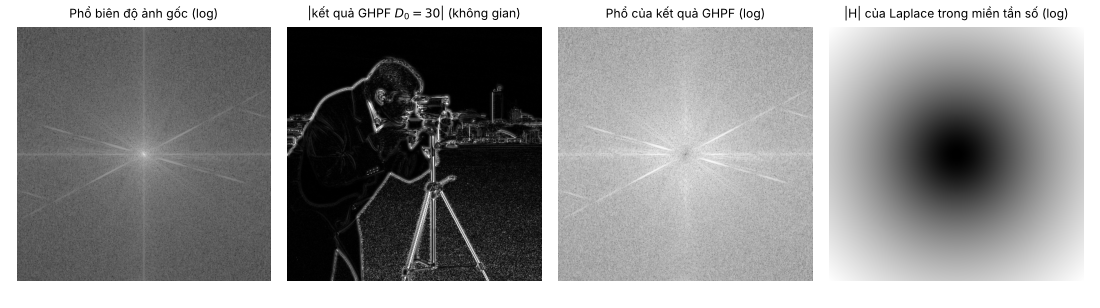
\includegraphics[width=\textwidth]{w7_edge_freq.png}
\caption{Từ trái sang: phổ ảnh gốc; ảnh kết quả lọc thông cao Gauss $D_0 = 30$ (lấy trị tuyệt đối); phổ của ảnh kết quả, năng lượng vùng tâm đã bị loại bỏ; $|H|$ của toán tử Laplace trong miền tần số.}
\label{fig:w7_edge_freq}
\end{figure}

% =====================================================================
\subsection{Bảng thống kê các phương pháp làm trơn và phát hiện biên trong miền tần số}
\label{subsec:w7_table}

\textit{Câu hỏi: Lập bảng thống kê các phương pháp làm trơn ảnh (lọc thông thấp) và phát hiện biên cạnh, làm sắc nét (lọc thông cao) trong miền tần số.}

Bảng~\ref{tab:w7_methods} thống kê $7$ phương pháp của mục 7.4 trong bài giảng, bổ sung $3$ phương pháp thường dùng (đánh dấu *). Trong bảng, $D = D(u, v)$ là khoảng cách tới tâm phổ. Mọi phương pháp đều thực hiện theo Giải thuật~\ref{alg:w7_filter}, độ phức tạp $O(PQ\log(PQ))$ do FFT, không phụ thuộc vào ``kích thước'' bộ lọc. Mỗi bộ lọc thông cao có thể suy từ bộ lọc thông thấp tương ứng: $H_{\text{cao}} = 1 - H_{\text{thấp}}$.

\begin{table}[!htbp]
\centering
\scriptsize
\caption{Các phương pháp lọc trong miền tần số}
\label{tab:w7_methods}
\renewcommand{\arraystretch}{1.3}
\begin{tabularx}{\textwidth}{|p{1.55cm}|p{2.6cm}|X|X|p{1.3cm}|}
\hline
\textbf{Phương pháp} & \textbf{Hàm truyền $H(u, v)$} & \textbf{Nguyên lý, tác dụng} & \textbf{Phản ứng phụ} & \textbf{Tham số} \\
\hline
\multicolumn{5}{|l|}{\textbf{Làm trơn — lọc thông thấp}} \\
\hline
Lý tưởng (ILPF) & $1$ nếu $D \le D_0$, $0$ nếu $D > D_0$ & Giữ nguyên tần số trong hình tròn bán kính $D_0$, xóa hẳn phần ngoài & Gợn sóng mạnh quanh biên (nhân không gian dạng $J_1(r)/r$); $D_0$ nhỏ thì rất mờ & $D_0$ \\
\hline
Butterworth (BLPF) & $\dfrac{1}{1 + (D/D_0)^{2n}}$ & Suy giảm dần, $H(D_0) = 0{,}5$; độ dốc theo $n$ & Gợn sóng tăng theo $n$ (không đáng kể khi $n \le 2$) & $D_0$, $n$ \\
\hline
Gauss (GLPF) & $e^{-D^2/2D_0^2}$ & Suy giảm mềm, $H(D_0) = 0{,}61$; tương đương lọc Gauss không gian & Không gợn sóng; tần số cắt không sắc & $D_0$ \\
\hline
\multicolumn{5}{|l|}{\textbf{Phát hiện biên, làm sắc nét — lọc thông cao}} \\
\hline
Lý tưởng (IHPF) & $0$ nếu $D \le D_0$, $1$ nếu $D > D_0$ & Xóa thành phần tần số thấp, giữ biên và chi tiết & Gợn sóng; biên bị nhân đôi; mất vùng đồng nhất (ảnh tối) & $D_0$ \\
\hline
Butterworth (BHPF) & $\dfrac{1}{1 + (D_0/D)^{2n}}$ & Như trên nhưng chuyển tiếp mềm & Ít gợn sóng; khuếch đại nhiễu & $D_0$, $n$ \\
\hline
Gauss (GHPF) & $1 - e^{-D^2/2D_0^2}$ & Chuyển tiếp mềm nhất, biên sạch & Không gợn sóng; khuếch đại nhiễu & $D_0$ \\
\hline
Laplace & $-4\pi^2\big[(u/M)^2 + (v/N)^2\big]$ (dịch tâm) & Đạo hàm bậc hai, $H \propto D^2$ tăng không giới hạn; điểm qua $0$ là biên; làm sắc: $g = f - c\,\nabla^2 f$ & Khuếch đại nhiễu tần số cao rất mạnh; cần chuẩn hóa kết quả & -- \\
\hline
\multicolumn{5}{|l|}{\textbf{Bổ sung}} \\
\hline
Nhấn tần số cao* & $a + b\,H_{\text{cao}}$, $a \ge 0$, $b > a$ & Làm sắc nét mà vẫn giữ nền: giữ một phần tần số thấp ($a$), nhấn tần số cao ($b$); tương đương lọc unsharp/high-boost & Khuếch đại nhiễu & $a$, $b$, $D_0$ \\
\hline
Đồng hình (homomorphic)* & $(\gamma_H - \gamma_L)\big(1 - e^{-cD^2/D_0^2}\big) + \gamma_L$ áp dụng cho $\ln f$ & Tách thành phần chiếu sáng (tần số thấp) và phản xạ (tần số cao): giảm độ chênh sáng, tăng tương phản chi tiết & Có thể tạo quầng sáng quanh biên & $\gamma_L$, $\gamma_H$, $c$, $D_0$ \\
\hline
Chắn khấc / chắn dải* & $\prod_k \big[1 - e^{-D_k^2/2D_0^2}\big]$ với $D_k$ là khoảng cách tới đỉnh nhiễu thứ $k$ & Xóa nhiễu tuần hoàn bằng cách đặt $H = 0$ tại các đỉnh nhiễu trên phổ (Hình~\ref{fig:w7_periodic}) & Xóa cả thành phần ảnh thật trùng tần số đỉnh nhiễu & Vị trí đỉnh, $D_0$ \\
\hline
\end{tabularx}
\end{table}
